\subsection*{Structural Analysis: Generation of MFP }

%\subsubsection*{a. Structure Subtraction and Counting}

%The main difference between CBC and CSBC method is that the latter uses structure subtraction operation to segregate the bits base on its significance. Structure subtraction is a procedure that is part of CSBC method that is devised by the researchers to extract the structural pattern dependence on position and neighbors. To CSBC method work, the following assumptions must be fulfilled; a) all of the compounds must undergo fragmentation via MFA to generate MP's; b) generated MP's was converted to matrix (1x2048); c) a neutral point must be assign, wherein, in this region the activity of compounds against HCT-116 is close to 0; d) difference in MP's of compounds located in neutral point vs the other region were considered to be significant bits; e) after structure subtraction, it will yield to formation of new MP's, the 1's, -1's and 0's were considered to be significant and non-significant bits(\autoref{fig:subtraction}. To account the positions and neighbors, the new MP's produced by structure subtraction were recompiled into clusters of HI-VLI, MI-VLI, LI-VLI, and NI-VLI. The produced clusters essentially contains the information about what are the unique bits found in subtracting the neutral point to the groups of compound with high and low bioactivity. For the case of HI-VLI, it is expected that the matrix elements equivalent to 1 are the unique positive bits (molecular fingerprints) that is responsible for the high bioactivity of the said compound, while the 0's and -1's are the non-significant and negative bits. The same assumption were used for MI-VLI, and LI-VLI, however, for NI-VLI, since these compounds have negative bioactivity the definition of 1's and -1's were inverted. Given that assumptions to be true, the researchers hypothesized that, if the bits have positional and neighbor dependency, therefore, they must be repeatedly observed across the clusters. To prove this hypothesis, the researchers try to find whether the top bits from HI-VLI were present in MI-VLI, LI-VLI, and NI-VLI. The results shows that the top bits from HI-VLI which are 1, 6, 8, 19, 51, 428, 598, 792, 857, 1085, 1155, 1556, 1863, 1917, 2039 and 1990, were also the top bits in MI-VLI, LI-VLI and NI-VLI. Therefore, these bits has the characteristics to positively and negatively affect the compounds bioactivity, which can only be attributed to their position and to the types of neighbor they have. 
%\vspace{-0.7cm}
\begin{figure}[h] % 'h' places the figure approximately here
	\centering
	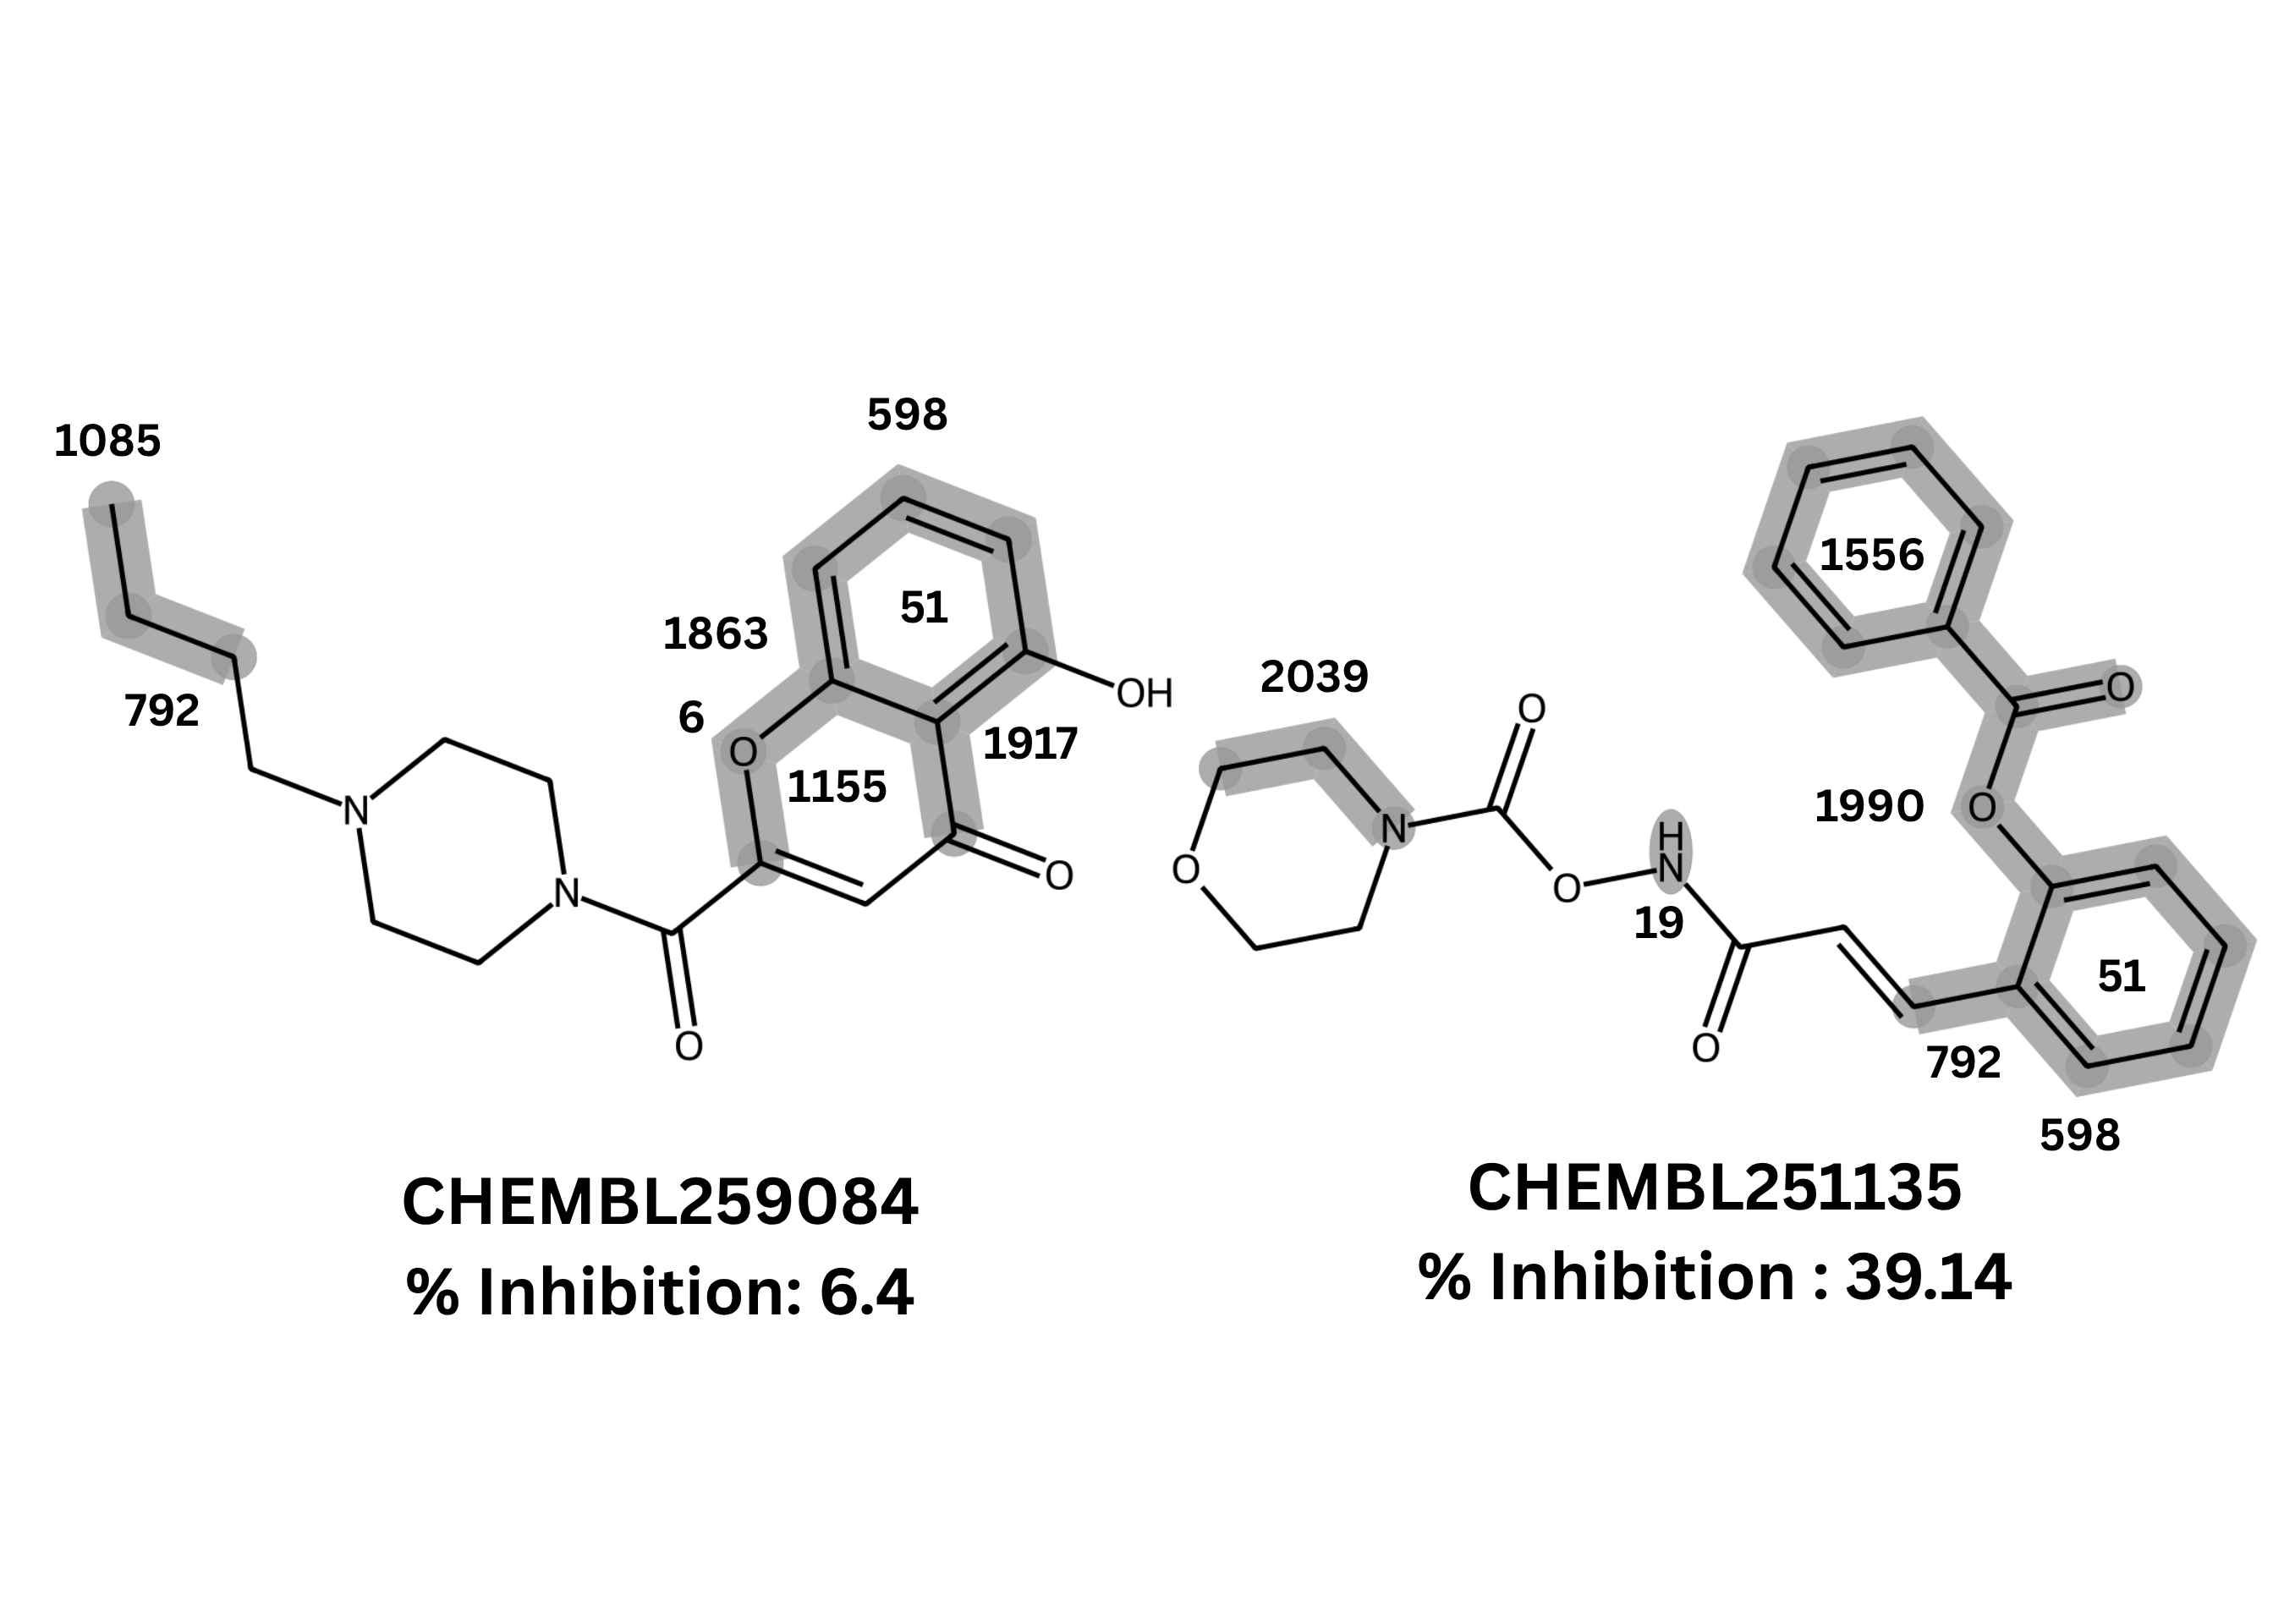
\includegraphics[width=0.8\textwidth]{6_4_vs_39_14_bits_visualization_bw.png} % Replace with your image filename
	\vspace{-0.7cm}
	\caption{Bits Detection of CSBC-ML:SAMPLE 1}
	\label{fig:bit_visualization_643914} % Optional: use \label for referencing
\end{figure}

\subsubsection*{a. Structural Analysis of Bits: Positions and Neighbors}

\begin{figure}[h] % 'h' places the figure approximately here
	\centering
	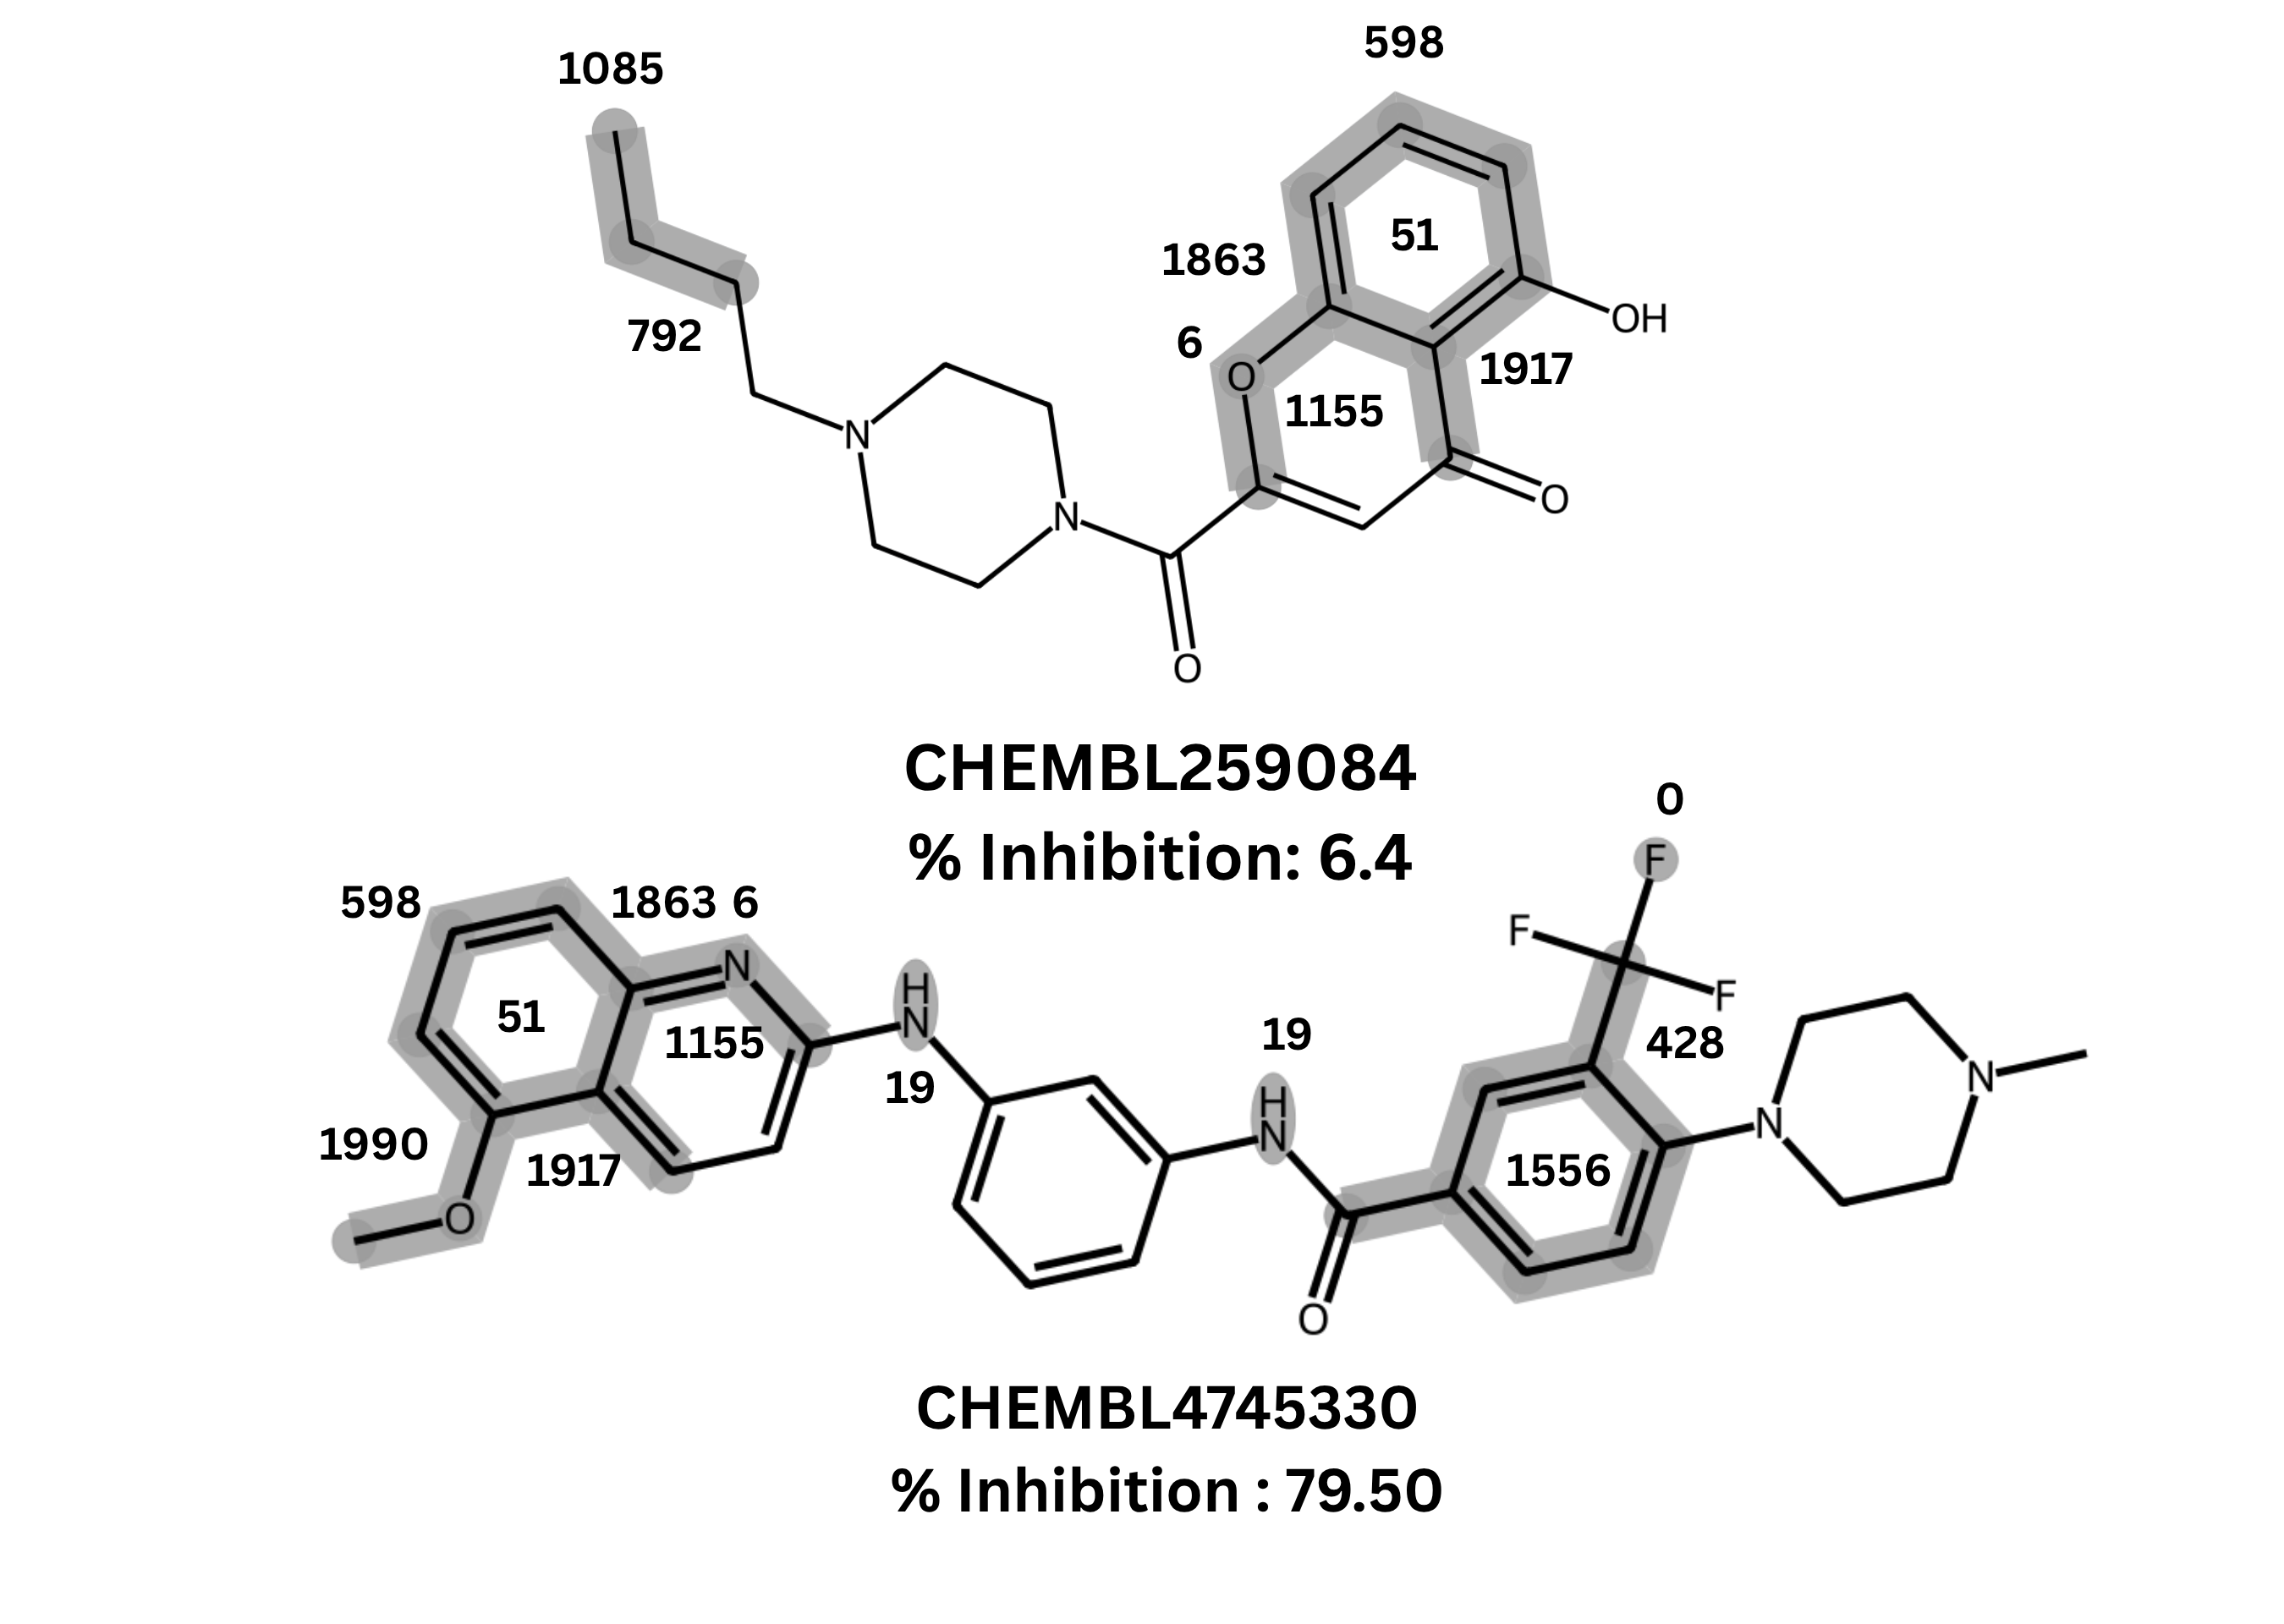
\includegraphics[width=0.7\textwidth]{79_5vs_6_4_bit_visualization_bw.png} % Replace with your image filename
	\caption{Bits Detection of CSBC-ML:SAMPLE 2}
	\vspace{-0.3cm}
	\label{fig:bit_visualization_7939} % Optional: use \label for referencing
\end{figure}

\begin{figure}[h] % 'h' places the figure approximately here
	\centering
	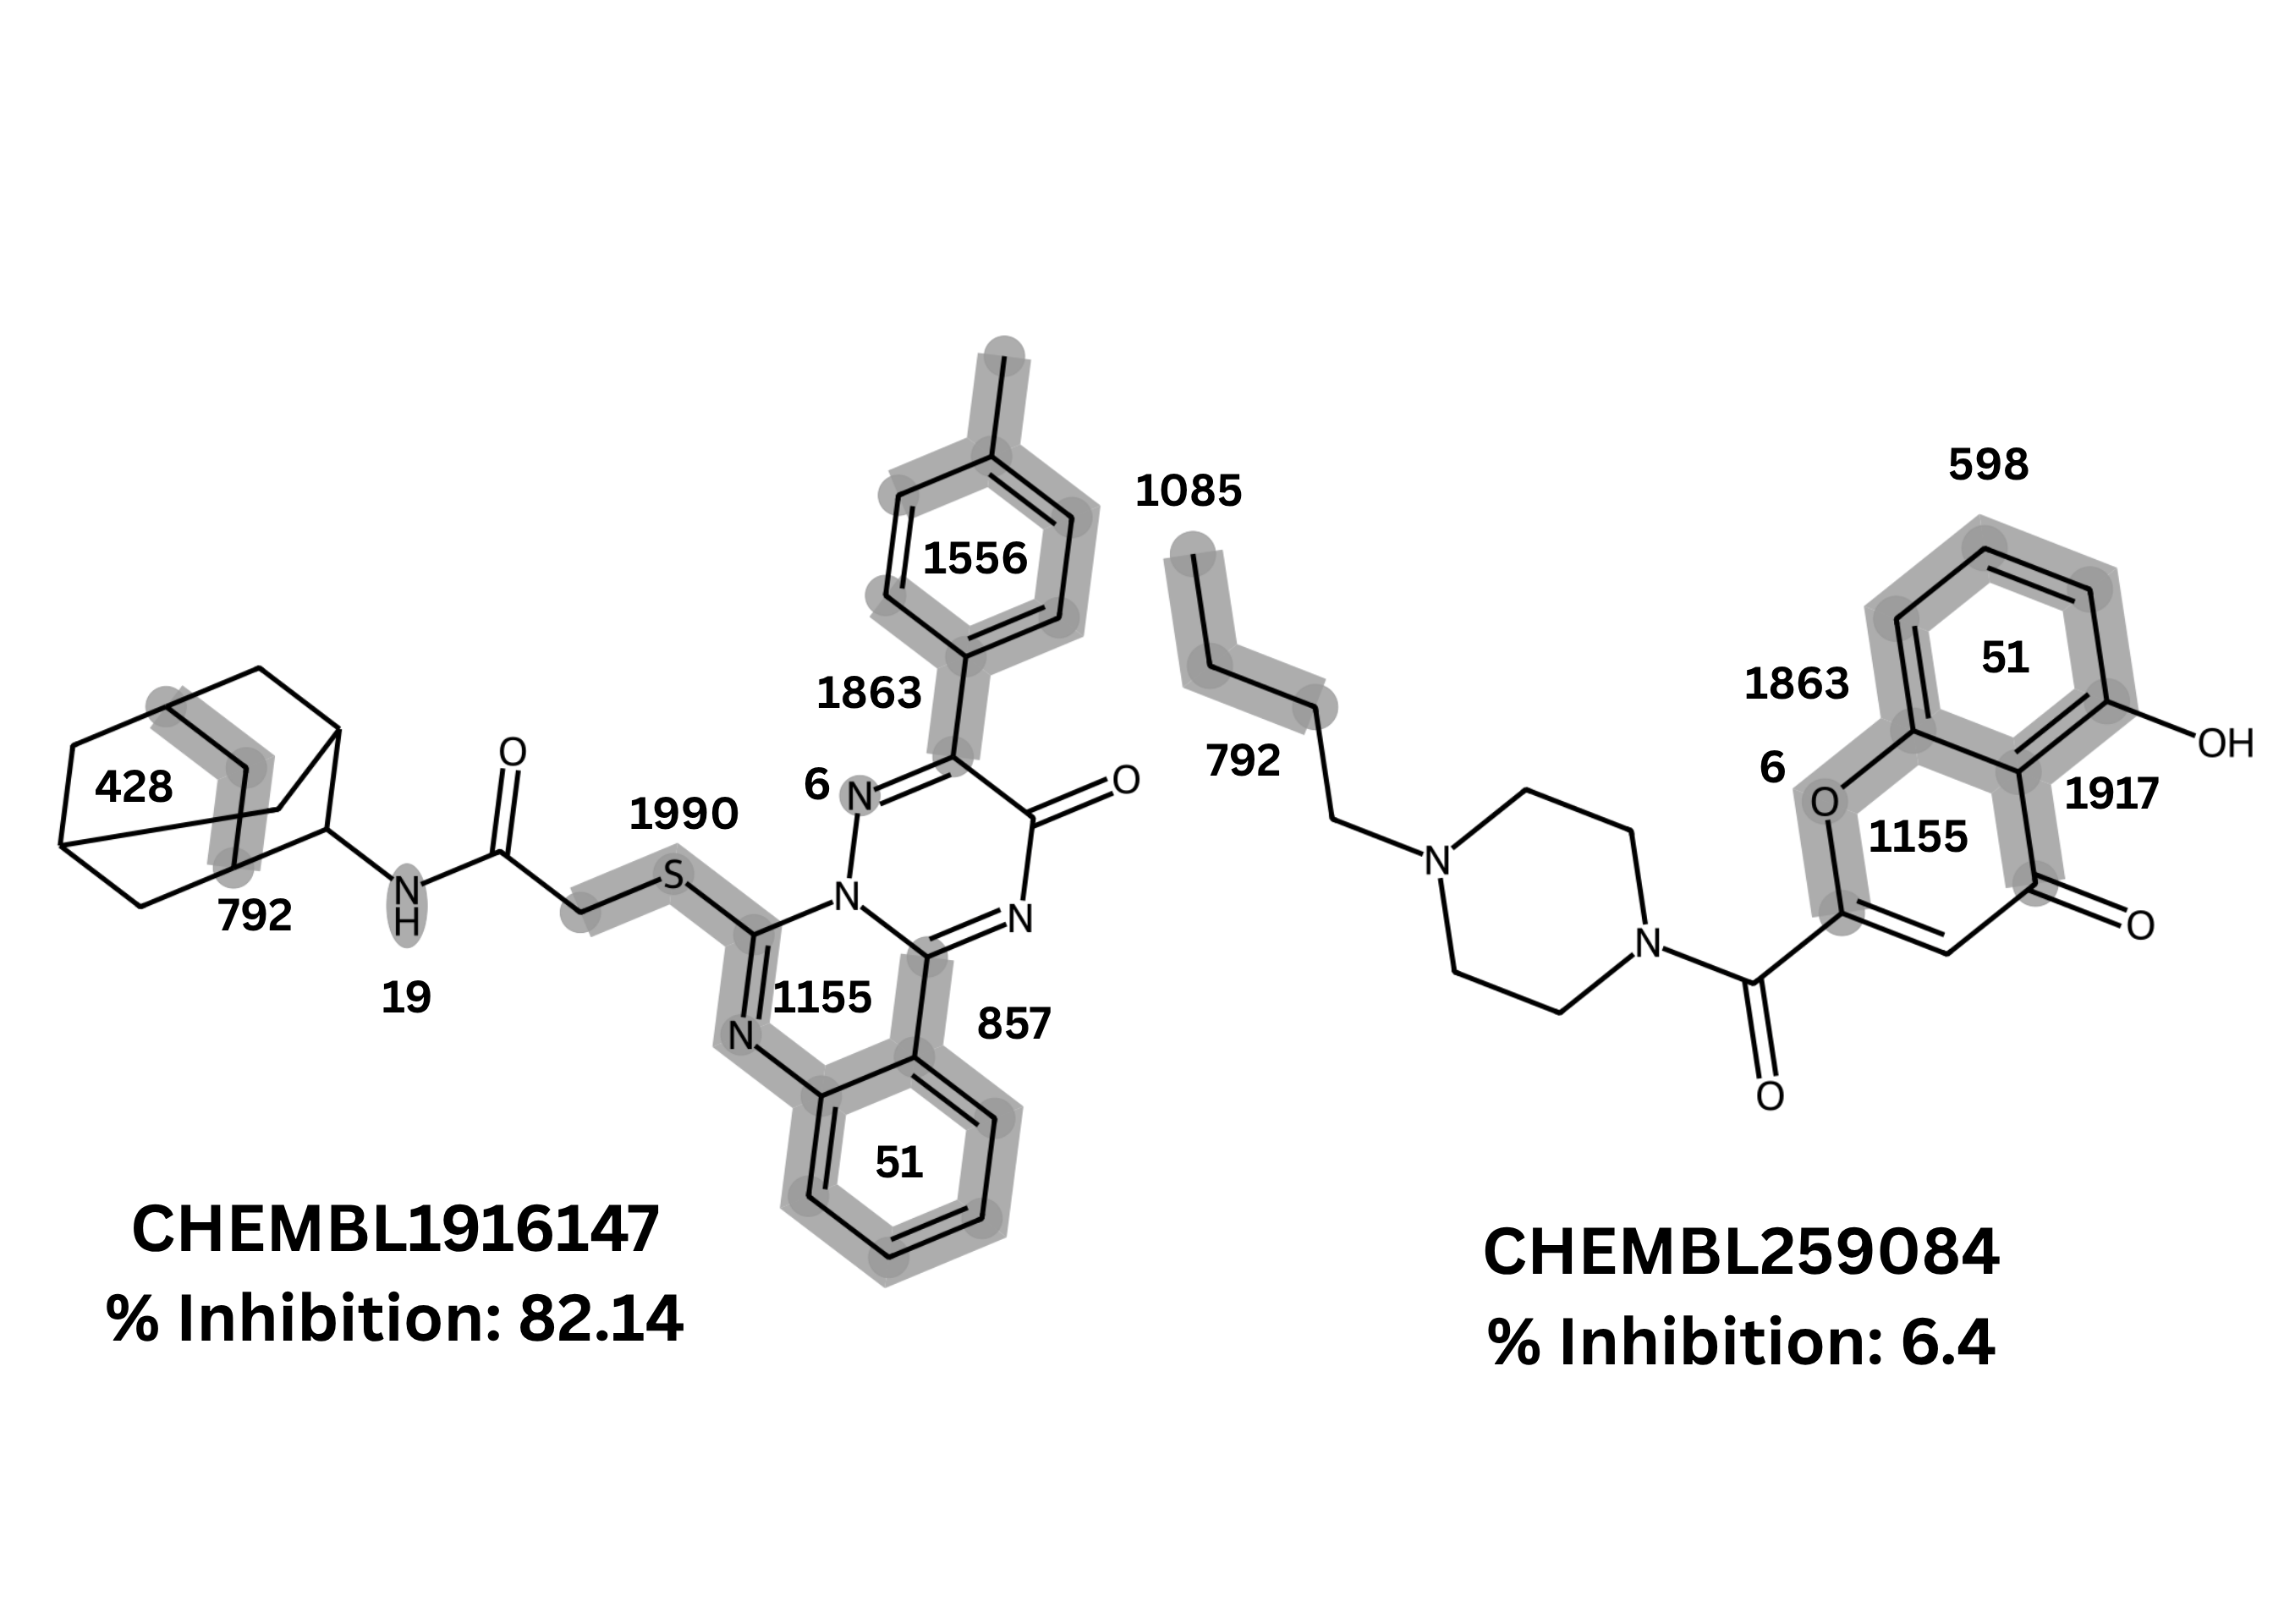
\includegraphics[width=0.7\textwidth]{82_14_vs_6_4_bits_visualization_bw.png} % Replace with your image filename
	\caption{Bits Detection of CSBC-ML:SAMPLE 3}
	\vspace{-0.3cm}
	\label{fig:bit_visualization_8264} % Optional: use \label for referencing
\end{figure}

\begin{figure}[htbp!] % 'h' places the figure approximately here
	\centering
	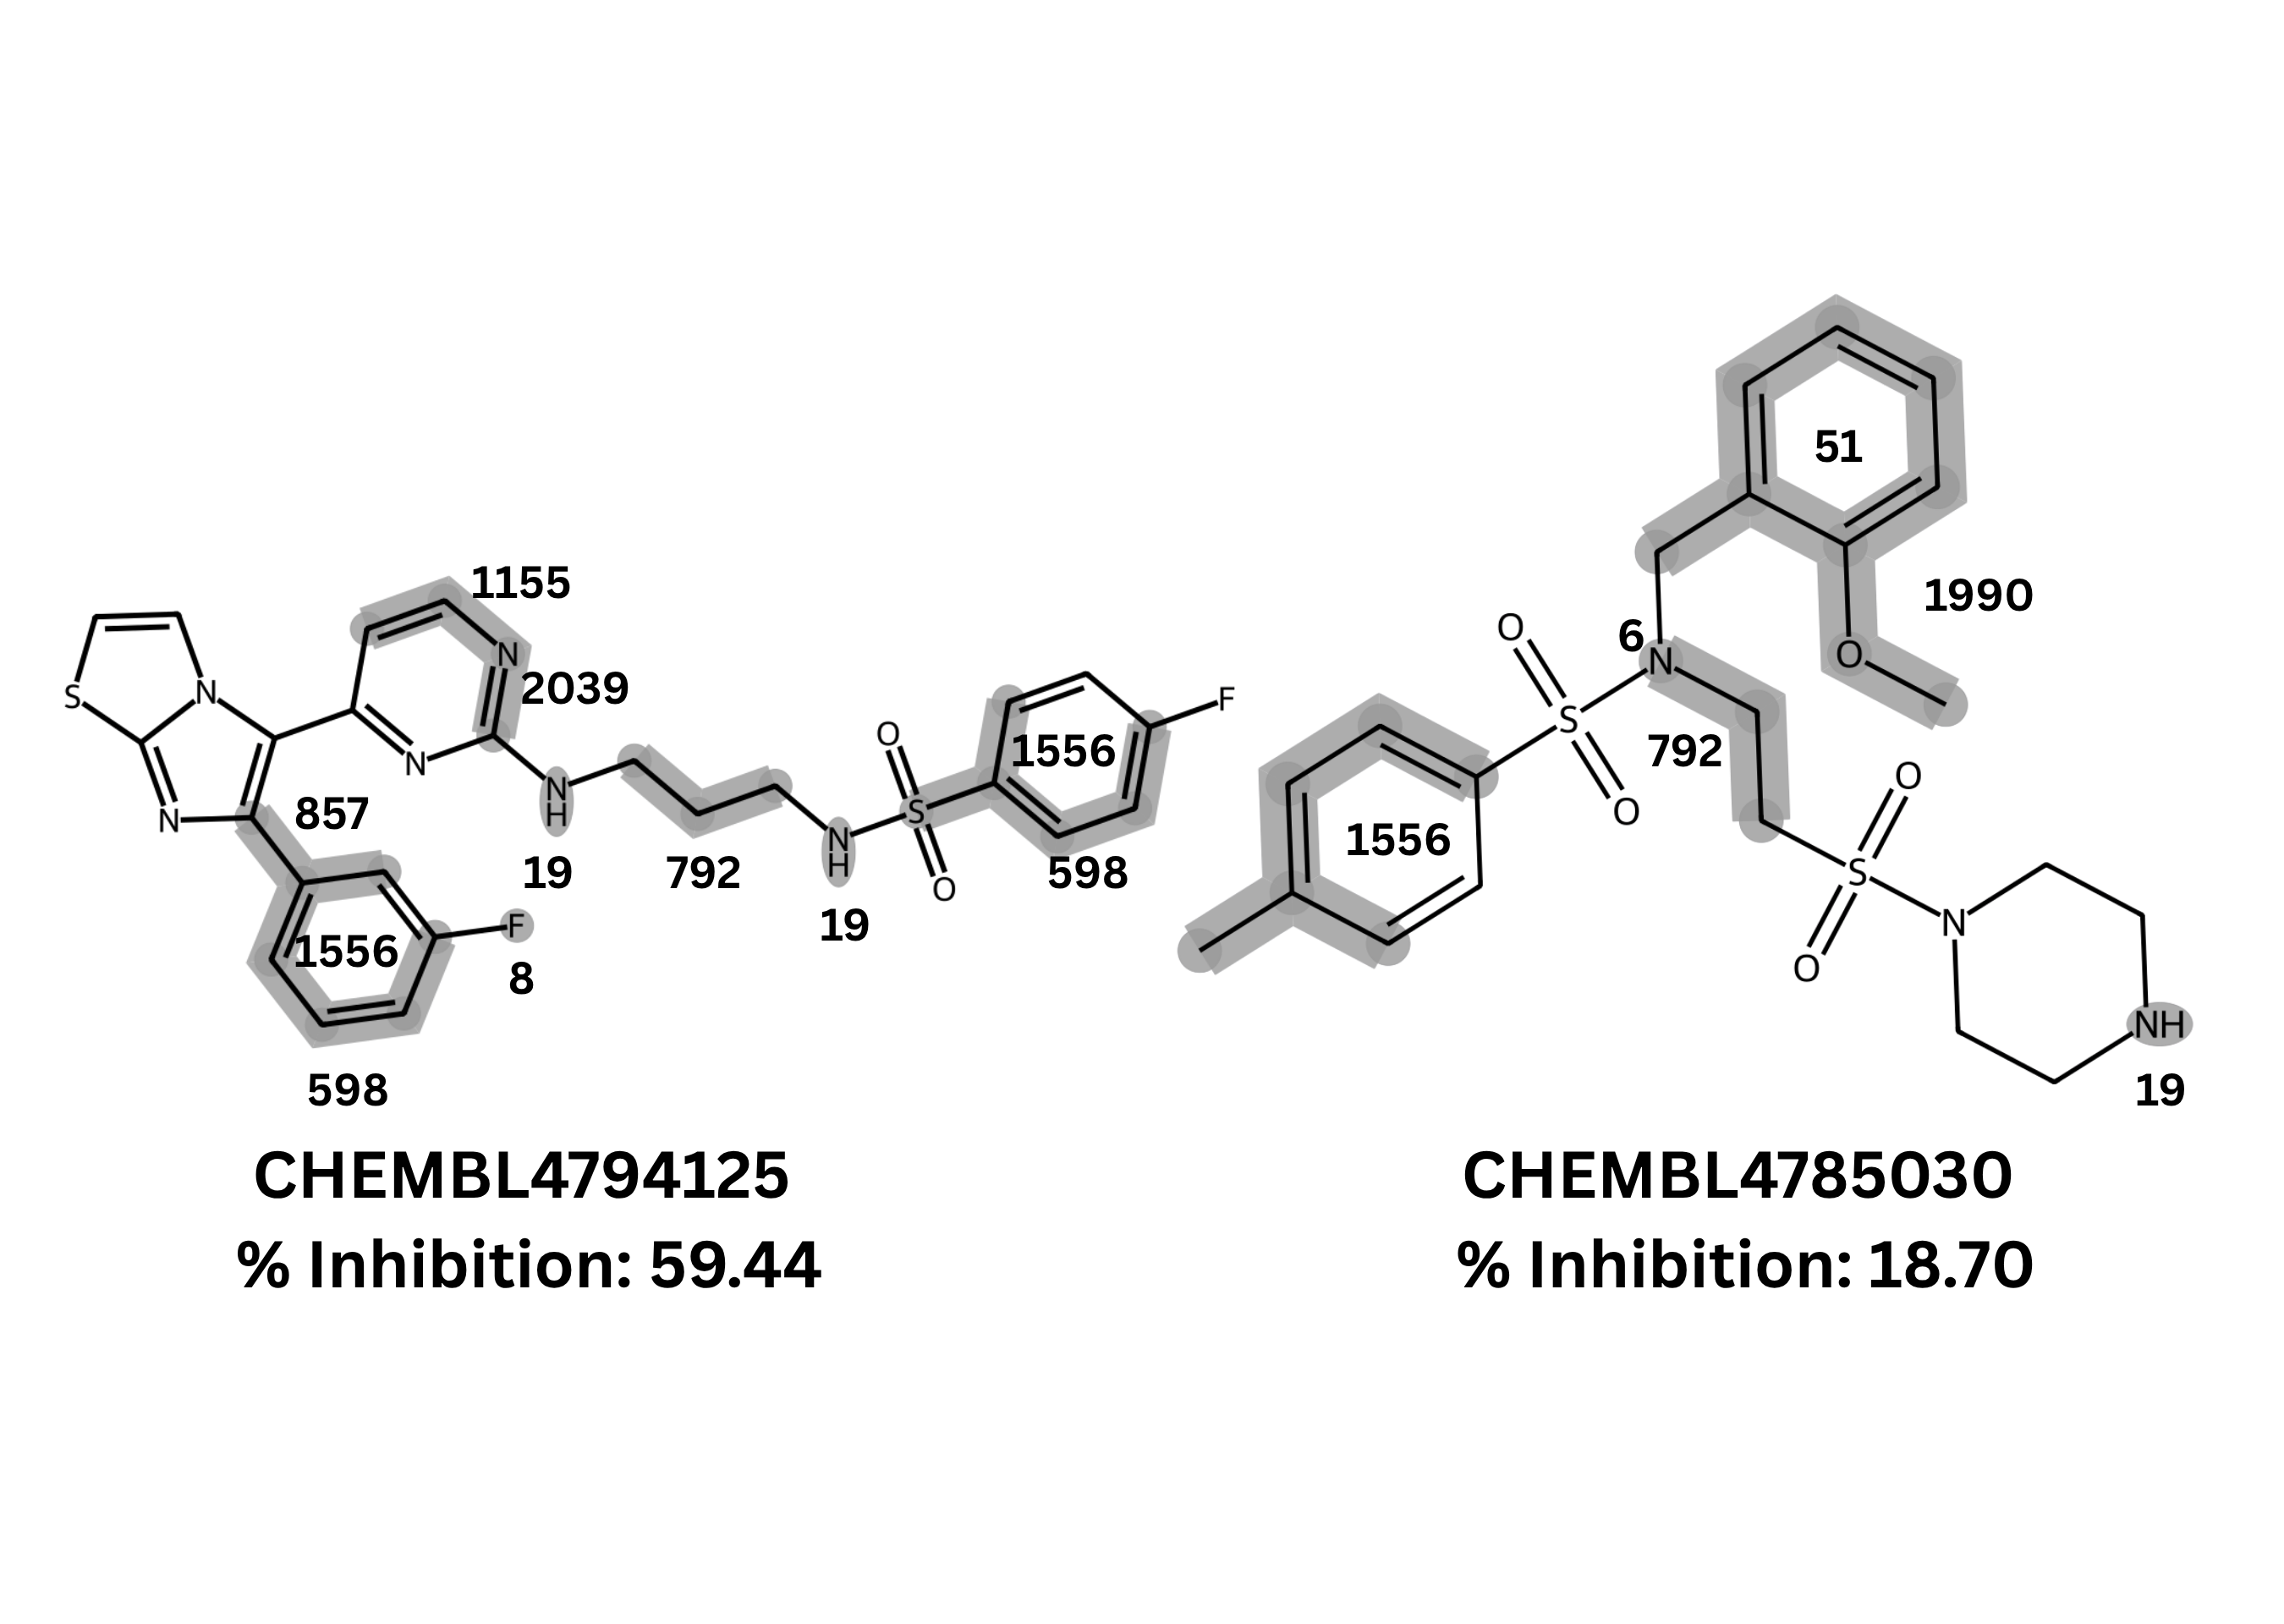
\includegraphics[width=0.8\textwidth]{3_403_mol_inhibition.png} % Replace with your image filename
	\caption{Bits Detection of CSBC-ML:SAMPLE 4}
	\vspace{-0.3cm}
	\label{fig:bit_visualization_5918} % Optional: use \label for referencing
\end{figure}

To validate bits positional and neighbor dependency, random molecules from the sample data set were taken, and subsequently fed to the CSBC-ML models (XGB, RF, SVM) for bit presence determination. However, this time the results were extracted as 2D image structure (png) file. \autoref{fig:bit_visualization_643914} - \ref{fig:bit_visualization_8264} shows some example of generated png files with bits of interest highlighted in grey. The figures show how the MLA perceived 2D structural queries during the training and testing periods. Inserted features (bits from CSBC) are highlighted and the irrelevant ones are not. It was observed that molecule CHEMBL259084 has an attributes of positive bits which are 1085, 792, 1863, 1155, 1917, 6, 51, and 598  but, its \% Inhibition against HCT-116 was only 6.4. On the other hand, CHEMBL251135 has also positive bits 2039, 19, 792, 598, 51, 1990, 1556, and its \% Inhibition was 39.14. Comparing the two molecules, the following can be observed: a) both of them have positive bits; b) they have common bits of 792, 51, 598; and c) the bioactivity of two molecules is significantly different. These observations can be explained by looking closely at their common bits. For instance in CHEMBL259084: bit 51 was positioned upward and close to bits 1863, 115 and 1917; bit 792 was situated far away from 51 and 598, close to 1085. On the other hand in CHEMBL251135, bit 51 was positioned downward and  close to 792, 598, 1990 and 1556 (\autoref{fig:bit_visualization_643914}). Another example is CHEMBL4745330,  %bits of 0, 6, 19, 51, 428, 598, 1155, 1556, 1863, 1917, and  1990,
comparing it to CHEMBL259084 they have common bits of 51, 598, 19, 1155, 1863, 1917, and 6 which are located at different positions but with almost the same neighbors --- only bit 1990 and 6 were added to it. (\autoref{fig:bit_visualization_7939}). These observations extends to other molecules such as CHEMBL1916147 (\% Inhibition 82.14) wherein bit 51 is positioned besides 857,1155, while bit 6 is near 1863, 1990, and 1156. In CHEMBL259084 they are positioned and neighbored differently (\autoref{fig:bit_visualization_8264}). These kind of observations were constantly observed throughout the randomized samples ---  \autoref{fig:bit_visualization_5918} shows the other subset of molecules. It is now apparent that the consolidation of similarities in position and structural neighborhood of bits from the cluster subtraction in CSBC were supported by observations on several structures that were visually inspected. From these results it can be drawn that qualitative structural analysis offers the visualization on the bits position and neighbor dependency, and that the results seems to validate all of the assumptions on significant bits dependency in position and neighbor. Furthermore, this might explain the compatibility of CSBC with XGB, RF and SVM models.
 
%Observing the structure of their common bits, 51 is positioned closed to bit 1863, 1155 and 1917 on an upward manner, bit 792 is situated far away from 51 and 598 but close to 1085 in CHEMBL259084, whereas, on CHEMBL251135, 51 is closed to 792, 598, 1990,1556, and protrude downward(\autoref{fig:bit_visualization_643914}). For other cases, CHEMBL4860630, has bits of 19, 1556, 1863, 1155, 1917, 2039, 1, 598 and 8, comparing it to CHEMBL251135 their common bits (598,19,1556,2039) were located at different positions and neighbors(\autoref{fig:bit_visualization_7939}). This extends to other molecules such as CHEMBL1916147 (\% Inhibition 82.14) wherein bit 51 is positioned besides 857,1155, while bit 6 is near 1863, 1990, and 1156 whereas in CHEMBL259084 they are positioned and neighbored differently (\autoref{fig:bit_visualization_8264}). Same kind of observations were seen throughout the randomized samples, hence, researchers conclude the following: a) qualitative structural analysis confirms and explains bits positional and neighbor dependency; b) the observation generated from it validates all of the assumptions on its compatibility as a feature on Xgb, RF and SVM models, wherein it is assumed that it will be forced to recognized the bits positional and neighbor dependency which in effect correcting its predictions; and c) the excellent performances of the CSBC-ML models is attributed to the correct selection of features. 
    

\subsubsection*{b. QSAR-ML Position and Neighbor Effects Rationalization}
CBC only relies on the presence and absence of MFP, and expects a linear relationship between the structure and target activity. Since it does not incorporate position and neighbor information, it was shown to result misclassifications. On the other hand, CSBC features were extracted and selected based on commonality across a given set of molecules. The top most common bits from CSBC are the collection of structures that are present in both active and inactive molecules, allowing non-linear mathematicals model combined to it implicitly accounts for the position and neighbors of the MFP. 

Among all of the mathematical models used in this study, logit performs the least in terms of confusion matrix parameters, AUC and ROC. This observation remains even if it is combined with CSBC features, and this can be attributed to the linearity of Logit, resulting to its inability to perceive position and neighbor differences of the bits. Therefore, it is difficult for the model to change its feature weights during the training and testing period, resulting to poor performance when compared to the other mathematical models. On the other hand, XGB, RF and SVM are mathematical models that have a self-correcting features. For XGB, the predictions are corrected by a log loss function, consisting of gradient and hessian functions that lets the model know far the predictions are from true values, which subsequently adjusts the step sized based on confidence in correction (\ref{eq:gradienthessian}). 

\begin{equation}  
   [ g_i = p_i - y_i ] [ h_i = p_i \times (1 - p_i) ]
    \label{eq:gradienthessian}
\end{equation}
where $g_{i}$ is the gradient, $h_{i}$ hessian, $p_{i}$ predicted probability and $y_{i}$ is the actual label (1 and 0). 

The model is designed to create initial predictions from a weak model, and from there the new trees were created and its leaves (feature weights) were updated based on the changes in gradient and hessian. The update on leaves will eventually stop when the log loss achieves its optimal solution. In this way, even though the features were not tweaked to have specific positions and neighbors, XGB theoretically is able to account for them during the learning process. Thus, this model combined with CSBC features excellently classified compounds activity and inactivity against HCT-116. In the case of RF, the predictions were adjusted based on a series of steps which include: a) reduction of over-fitting using multiple trees; b) introduction of randomness to improve generalization; and c) Handling Out-of-bag (OOB) predictions. This method uses various trees wherein features were split. This technique of handling data gives the model an advantage of learning new structural patterns from each trees. The average of trees will be used as the predicted value when a query is placed. There is then a high chance that the structural position and neighbors were among the several possible parameters that were learned by the trees during the learning process. 

For SVM, the predictions were adjusted based on the loss, support vectors and weight parameter optimization. Loss is the sum of errors during misclassification, whereas support vectors adjust the hyperplane boundary of features during the learning process. Hyperplanes are the collection of features that are spatially bounded, and adjusted when the support vectors detects new pattern during the learning process. This leads to the possibility of the model to learn bit dependency on position and neighbor during training and testing period.

%\subsubsection*{b. Structural Analysis of Bits: Positions and Neighbors }
%To further explain and understand the compatibility of CSBC with Xgb, RF and SVM, the researchers take random molecules from the sample data set, and then they introduce it to CSBC-ML model for bit presence identification, however, this time the results from it were extracted as png file for manual structural analysis. Through structural inspection, researchers notice that there are common bits that were present both on active and inactive compounds, however, their positions\footnote{define as location of the molecule in a given space, can also to be interpreted as conformation} and neighbors were different. The researchers hypothesized that modification on the common bits, could lead to a positive, moderate, and negative effects on compounds bioactivity against HCT-116. To give a context, (\autoref{fig:bit_visualization_643914}) presents two among of the many compounds that were randomly selected for structural analysis. The model highlighted significant bits that were identified to have relationship with \% Inhibition activity against HCT-116. From the 2D-structures, researchers hypothesized that in order for CHEMBL259084 to become more active, the position of bits 51 should be shifted from axial to equatorial, which can be achieved through ring opening in bit 1155, which cause to transform bit 6 and 1863 to form bit 1990. In other cases, changes in the highlighted part of the structures results to drastic change in bioacitivity (\autoref{fig:bit_visualization_7939} to \autoref{fig:bit_visualization_8264})    



%From these visualization, the abstract weight assignment of the Xgb, RF, and SVM models were partially understood. The information generated from here will be further used to create a unified rules that will simplify drug screening. Hence, the researchers aim to conduct a second part of this study, wherein the number of data sets will be increased to test the robustness, stability and accuracy of the developed CSBC-ML on classifying drugs acitivity or inactivity against HCT-116 and other cancer cell line as well.